%!TEX root = ../../thesis.tex

\section{Our System: \sys{DrQA}}
\label{sec:drqa}

\subsection{An Overview}

In the following we describe our system \sys{DrQA}, which focuses on answering questions using English Wikipedia as the unique knowledge source for documents. We are interested in building a general-knowledge question answering system, which can answer any sort of factoid questions where the answer is contained in and can be extracted from Wikipedia.

There are several reasons that we choose to use Wikipedia: 1) Wikipedia is a constantly evolving source of large-scale, rich, detailed information that could facilitate intelligent machines. Unlike knowledge bases (KBs) such as \sys{Freebase} or \sys{DBPedia}, which are easier for computers to process but too sparsely populated for open-domain question answering, Wikipedia contains up-to-date knowledge that humans are interested in. 2) Many reading comprehension datasets (e.g., \sys{SQuAD}) are built on Wikipedia so that we can easily leverage these resources and we will describe it soon. 3) Generally speaking, Wikipedia articles are clean, high-quality and well-formed and thus they are highly useful resources for open domain question answering.

Using Wikipedia articles as the knowledge source causes the task of question answering (QA) to combine the challenges of both large-scale open-domain QA and of machine comprehension of text. In order to answer any question, one must first retrieve the few relevant articles among more than 5 million items, and then scan them carefully to identify the answer. This is reminiscent of how classical TREC QA systems worked, but we believe that neural reading comprehension models will play a crucial role of \ti{reading} the retrieved articles/passages to obtain the final answer. As shown in Figure \ref{fig:drqa-system}, our system essentially consists of two components: (1) the \sys{Document Retriever} module for finding relevant articles and (2) a reading comprehension model, \sys{Document Reader}, for extracting answers from a single document or a small collection of documents.

Our system treats Wikipedia as a collection of articles and does not rely on its internal graph structure. As a result, our approach is generic and could be switched to other collections of documents, books, or even daily updated newspapers. We detail the two components next.

\subsection{Document Retriever}
\label{sec:doc-retriever}
Following classical QA systems, we use an efficient (non-machine learning) document retrieval system to first narrow our search space and focus on reading only articles that are likely to be relevant. A simple inverted index lookup followed by term vector model scoring performs quite well on this task for many question types, compared to the built-in ElasticSearch based Wikipedia Search API \cite{gormley2015elasticsearch}. Articles and questions are compared as TF-IDF weighted bag-of-word vectors.

We further improve our system by taking local word order into account with n-gram features. Our best performing system uses bigram counts while preserving speed and memory efficiency by using the hashing of \cite{weinberger2009feature} to map the bigrams to $2^{24}$ bins with an unsigned \emph{murmur3} hash.

We use the \sys{Document Retriever} as the first part of our full model, by setting it to return 5 Wikipedia
articles given any question. Those articles are then processed by the \sys{Document Reader}.


\begin{figure}[t]
\begin{center}
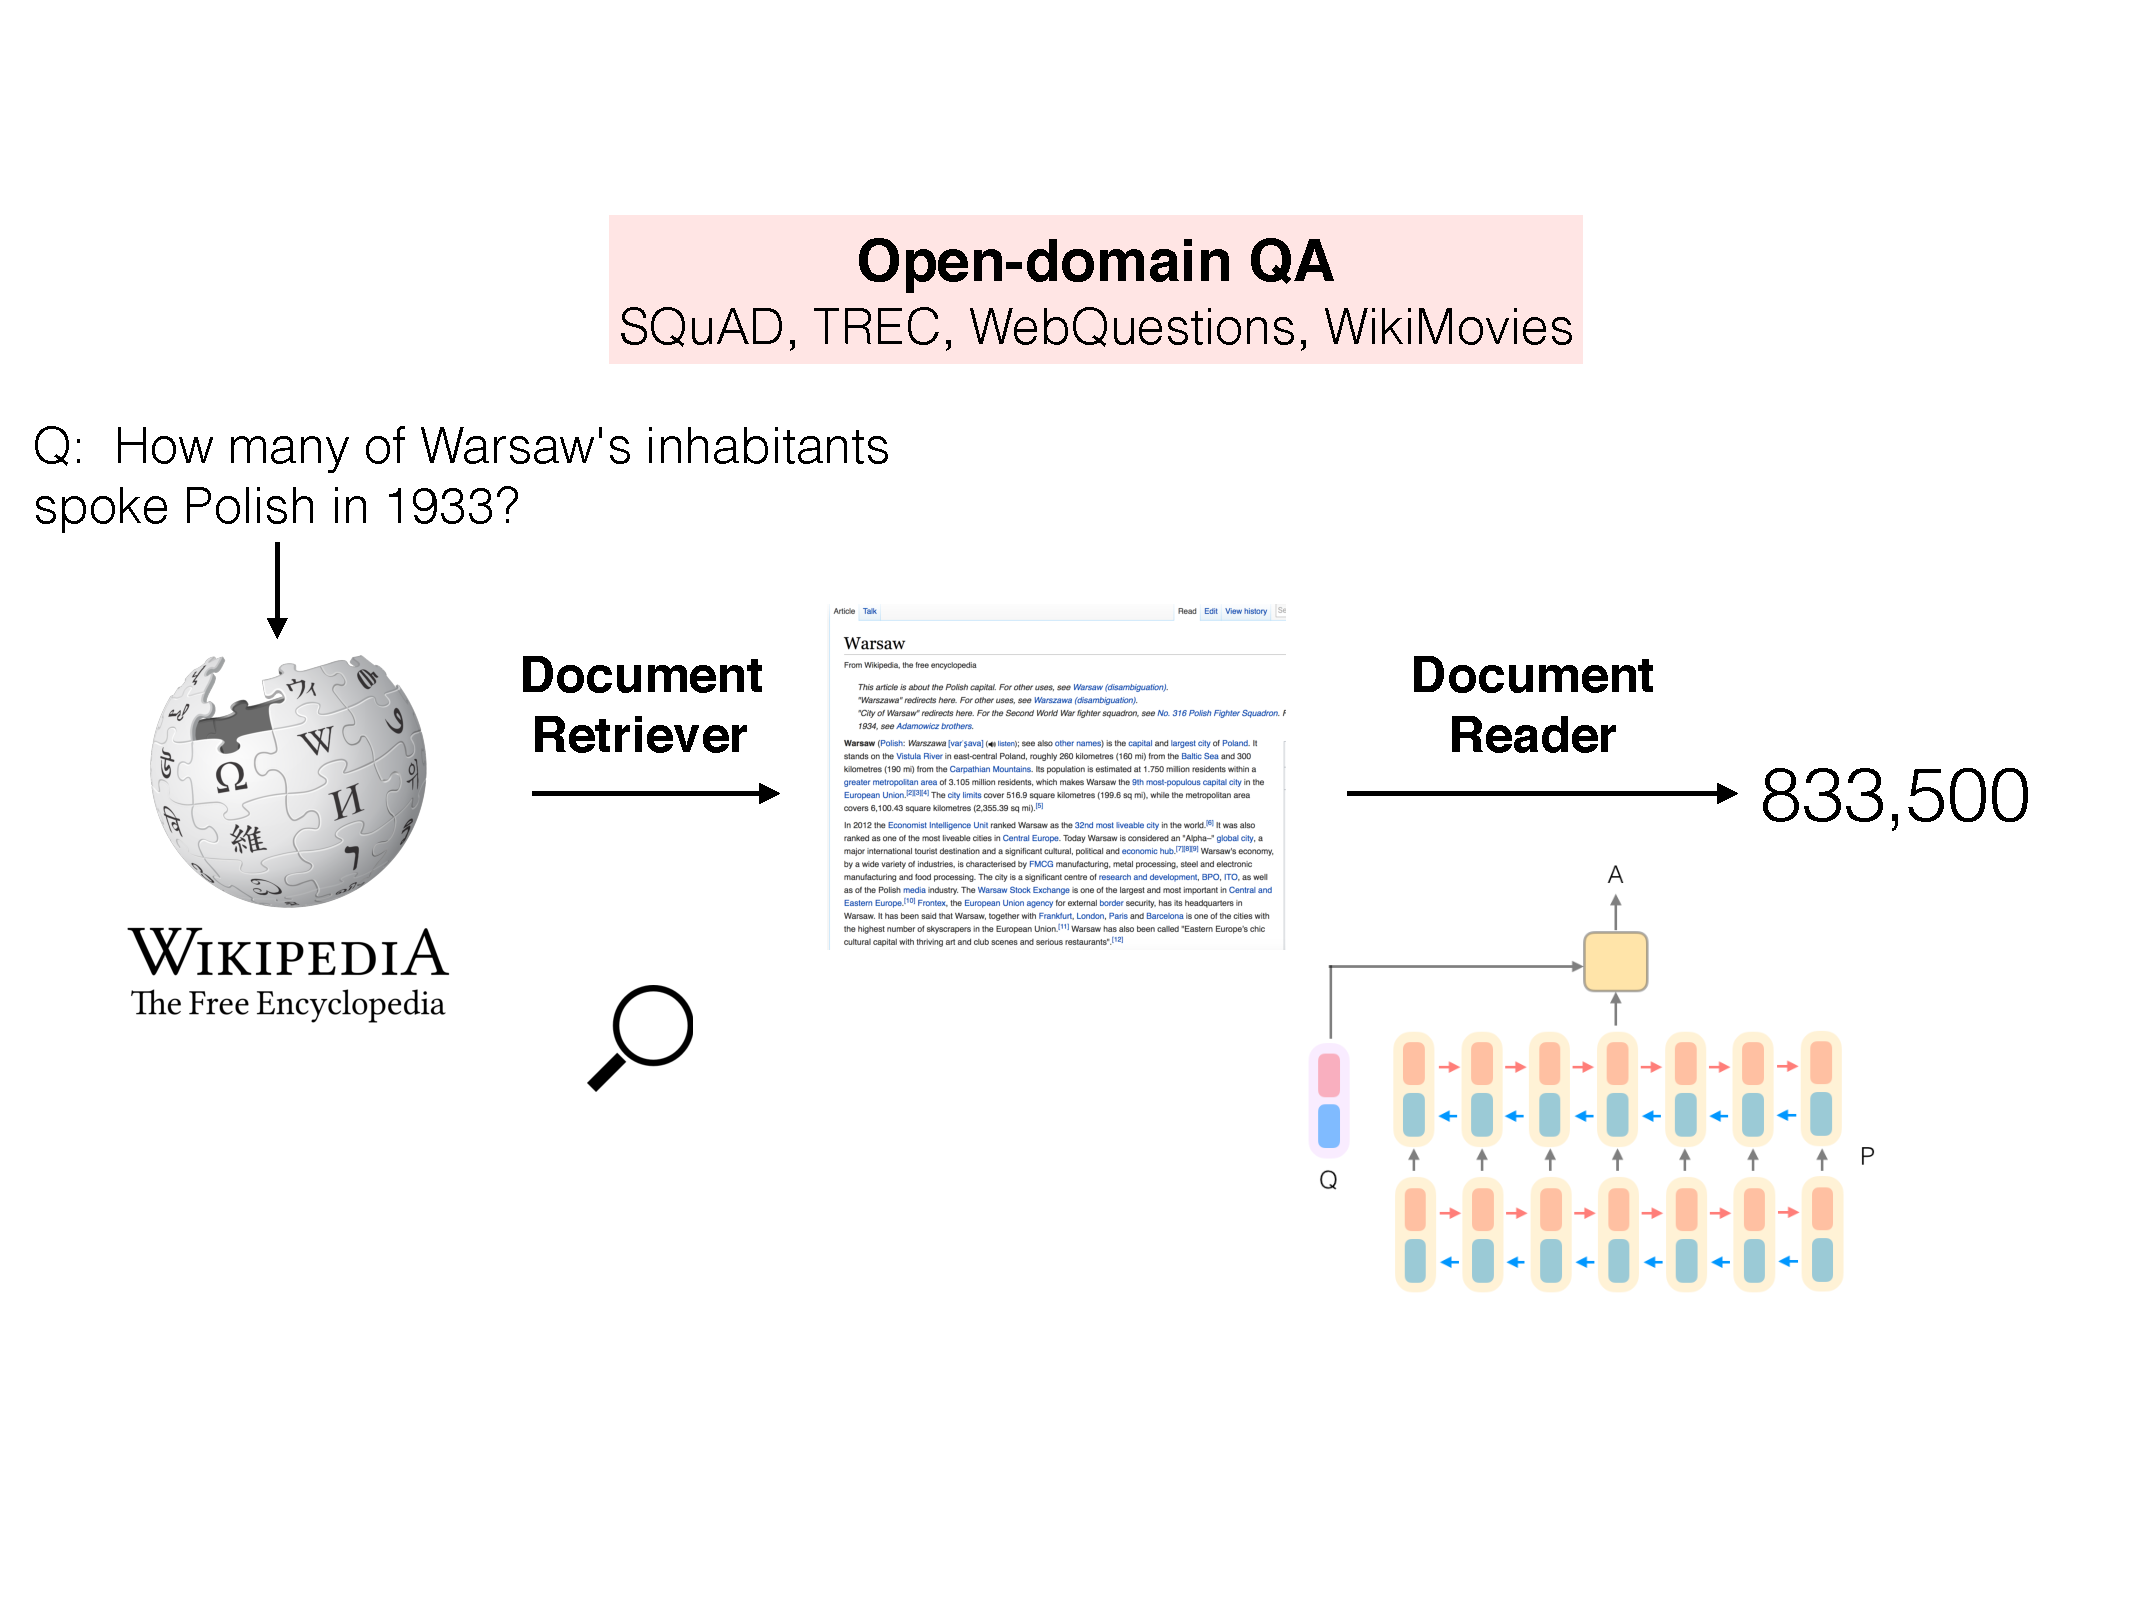
\includegraphics[height=8cm]{img/drqa_system.pdf}
\end{center}
\longcaption{An overview of DrQA system}{\label{fig:drqa-system} An overview of our question answering system DrQA.}
\end{figure}

\subsection{Document Reader}
The \sys{Document Reader} takes the top 5 Wikipedia articles and aims to read all the paragraphs and extracts the possible answers from them. This is exactly the setup as we did in span-based reading comprehension problems, and the \sys{Stanford Attentive Reader} model that we described in Section~\ref{sec:sar} can be directly plugged into this pipeline.

We apply our trained \sys{Document Reader} for each single paragraph that appears in the top 5 Wikipedia articles and it predicts an answer span with a confidence score. To make scores compatible across paragraphs in one or several retrieved documents, we use the unnormalized exponential and take argmax over all considered paragraph spans for our final prediction. This is just a very simple heuristic and there are better ways to aggregate evidence over different paragraphs. We will discuss future work in Section~\ref{sec:openqa-future}.

\subsection{Distant Supervision}
We have built a complete pipeline which integrates a classical retrieval module and our previous neural reading comprehension component. The remaining key question is how can we train this reading comprehension module for the open-domain question answering setting?

The most direct approach is just to reuse the SQuAD dataset~\cite{rajpurkar2016squad} as the training corpus, which was also built on top of Wikipedia paragraphs. However, this approach is limited in the following ways:

\begin{itemize}
    \item
        As we discussed earlier in Section~\ref{sec:future-datasets}, the questions in \sys{SQuAD} were crowdsourced after the annotators see the paragraphs to ensure they can be answered by a span in the passage. This distribution is quite specific and different from that of real-world question-answering when people have a question in mind first and try to find out he answers from the Web or other sources.
    \item
        Many \sys{SQuAD} questions are indeed context-dependent. For example, a question is \ti{What individual is the school named after?} posed on one passage of the Wikipedia article \ti{Harvard University}, or another question is \ti{What did Luther call these donations?} based on a passage that describes \ti{Martin Luther}. Basically, these questions cannot be understood by themselves and thus are useless for open-domain QA problems. \newcite{clark2018simple} estimated around 32.6\% of the questions in \sys{SQuAD} are either document-dependent or passage-dependent.
    \item
        Finally, the size of SQuAD is rather small (80k training examples). It should further improve the system performance if wen can collect more training examples.
\end{itemize}

To overcome these problems, we propose a procedure to automatically create additional training examples from other question answering resources. The idea is to re-use the efficient information retrieval module that we built: if we already have a question answer pair $(q, a)$ and the retrieval module can help us find a paragraph relevant to the question $q$ and the answer segment $a$ appears in the paragraph, then we can create a \ti{distantly-supervised} training example in the form of a $(p, q, a)$ triple for training the reading comprehension models:

\begin{eqnarray}
   & f: (q, a) \Longrightarrow (p, q, a) \\
    & \text{ if } p \in \text{ Document\_Retriever }(q) \text{ and } a \text{ appears in } p \nonumber
\end{eqnarray}

This idea is a similar spirit to the popular approach of using distant supervision (DS) for relation extraction \cite{mintz2009distant} \footnote{The idea for relation extraction is to pair textual mentions which contain the two entities which is known as a relation between them in an existing knowledge base.}. Despite that these examples can be noisy to some extent, it offers a cheap solution to create distantly supervised examples for open-domain question answering and will be a useful addition to \sys{SQuAD} examples. We will describe the effectiveness of these distantly supervised examples in Section~\ref{sec:drqa-eval}.
